\subsection{External interface requirements}
\subsubsection{User interfaces}
There are two categories of users that have different interface requirements:
\begin{itemize}
	\item {\bfseries Customers}\\
	Customers belong to all demographics so a user friendly interface is needed. The customer is presented with a main menu which allows him/her to:
	\begin{itemize}
		\item line up immediately (immediate reservation) at a specific store
		\item book a visit (future reservation) at a specific store
		\item view and delete existing reservations
	\end{itemize}
	The customer will receive a notification when it is time for him/her to depart to reach the shop.\\\\
	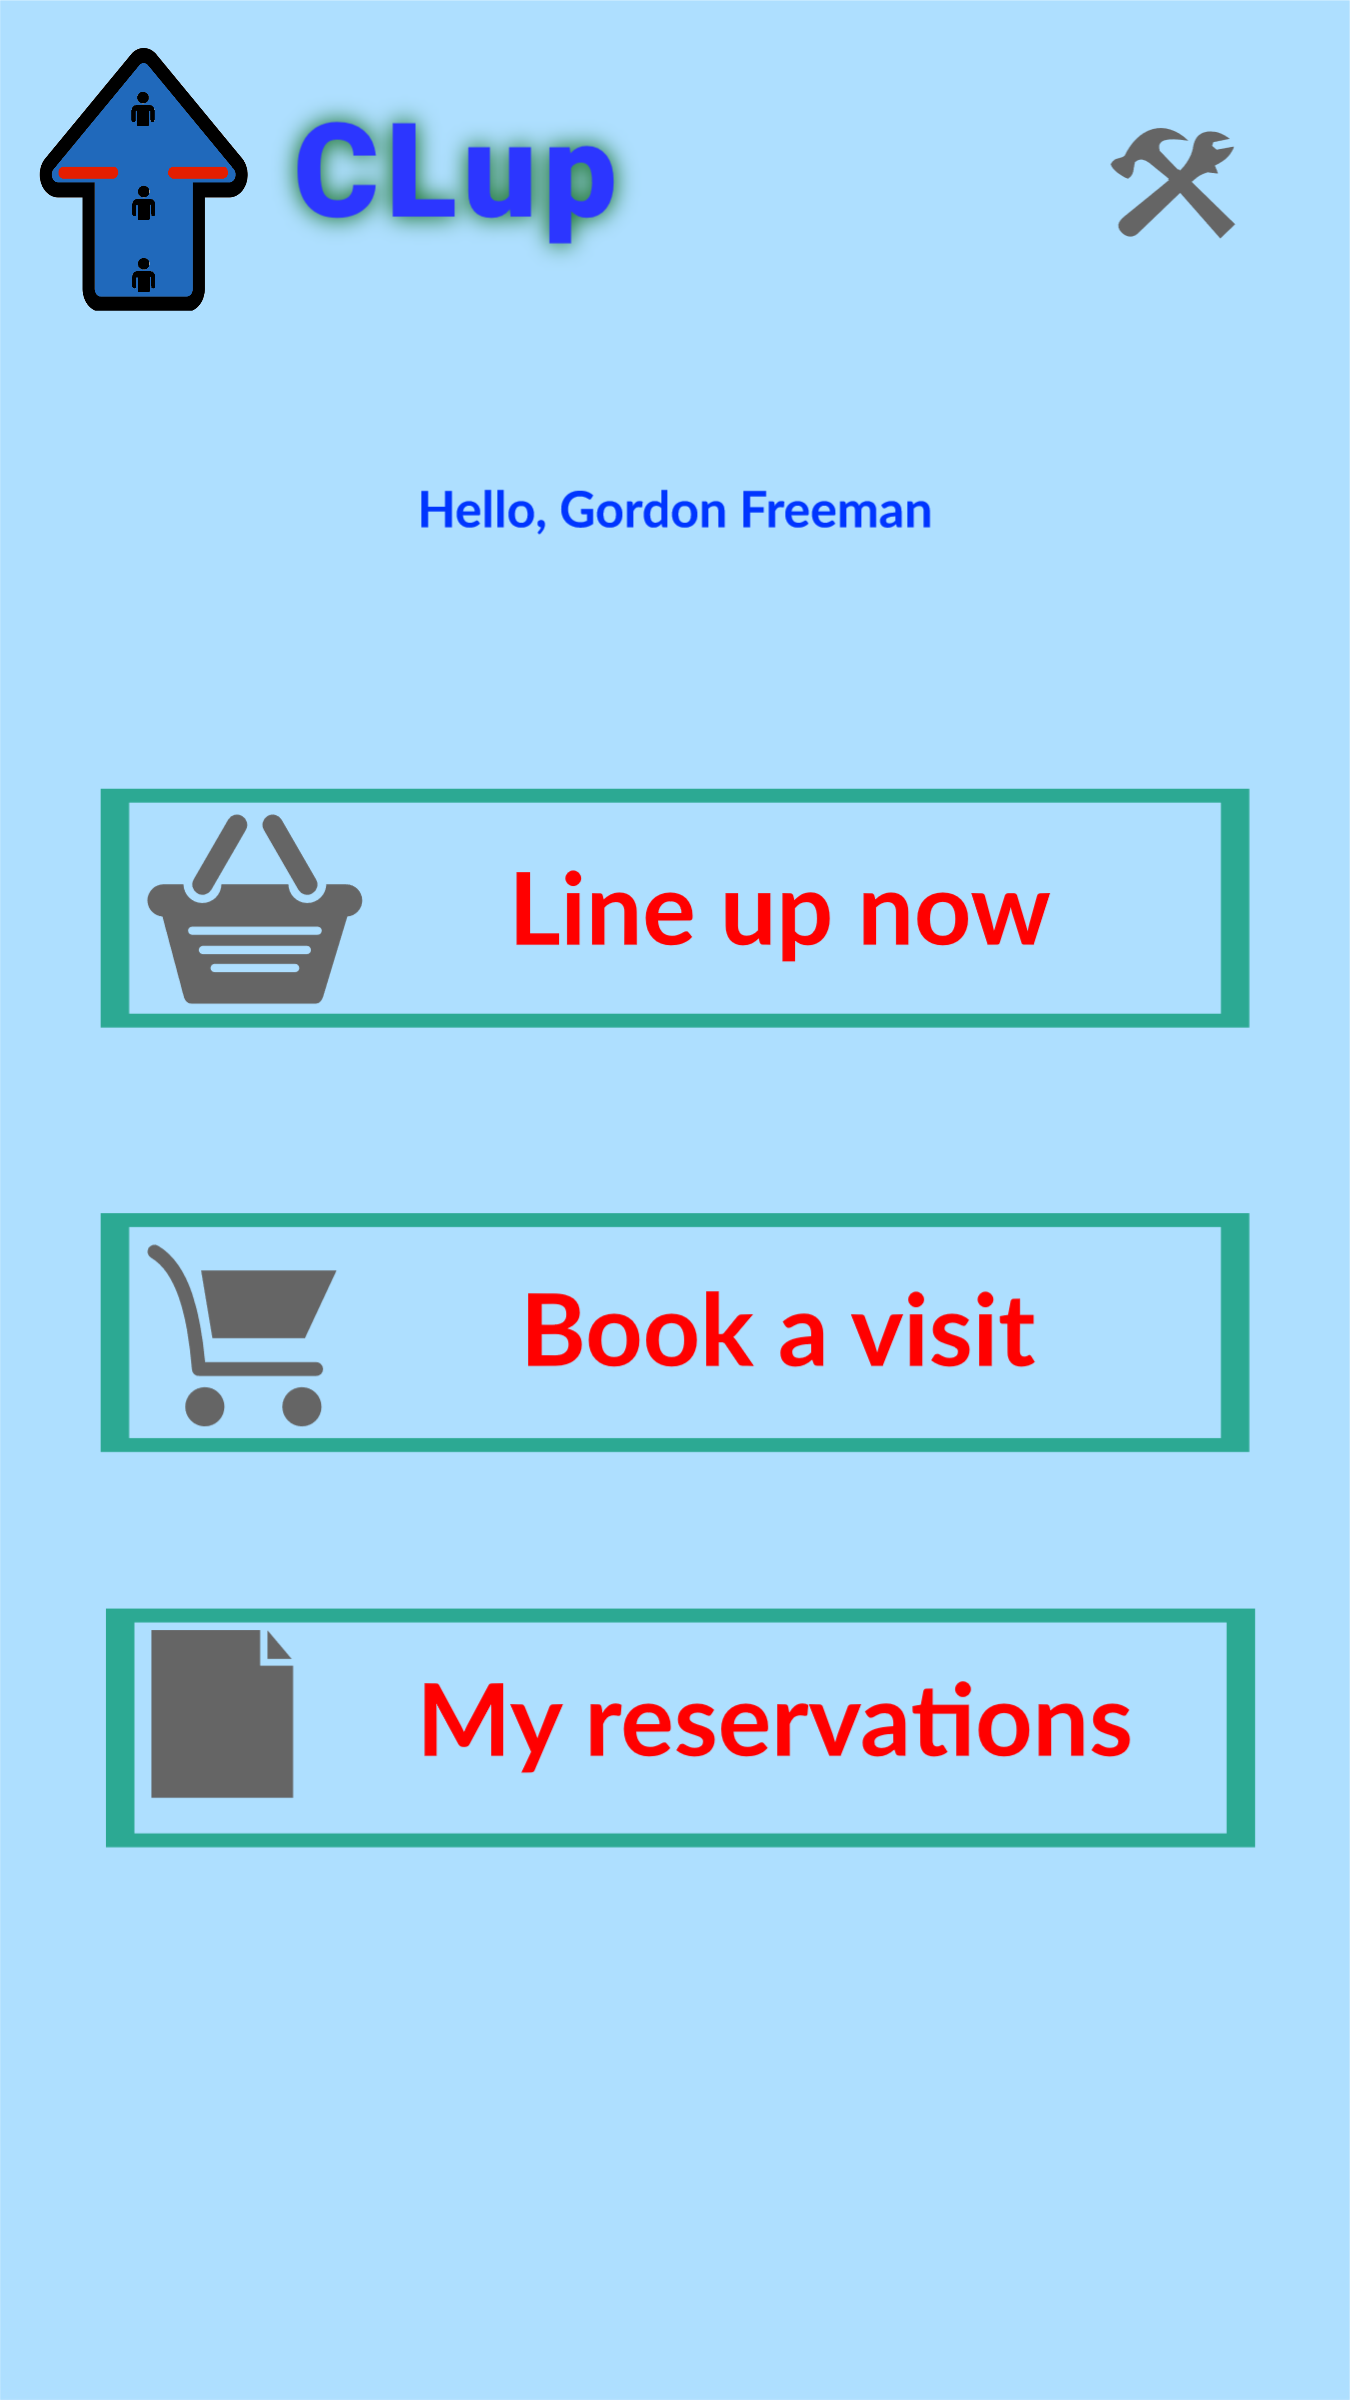
\includegraphics[scale=0.1]{Images/MainMenuCustomer.png}
	\qquad
	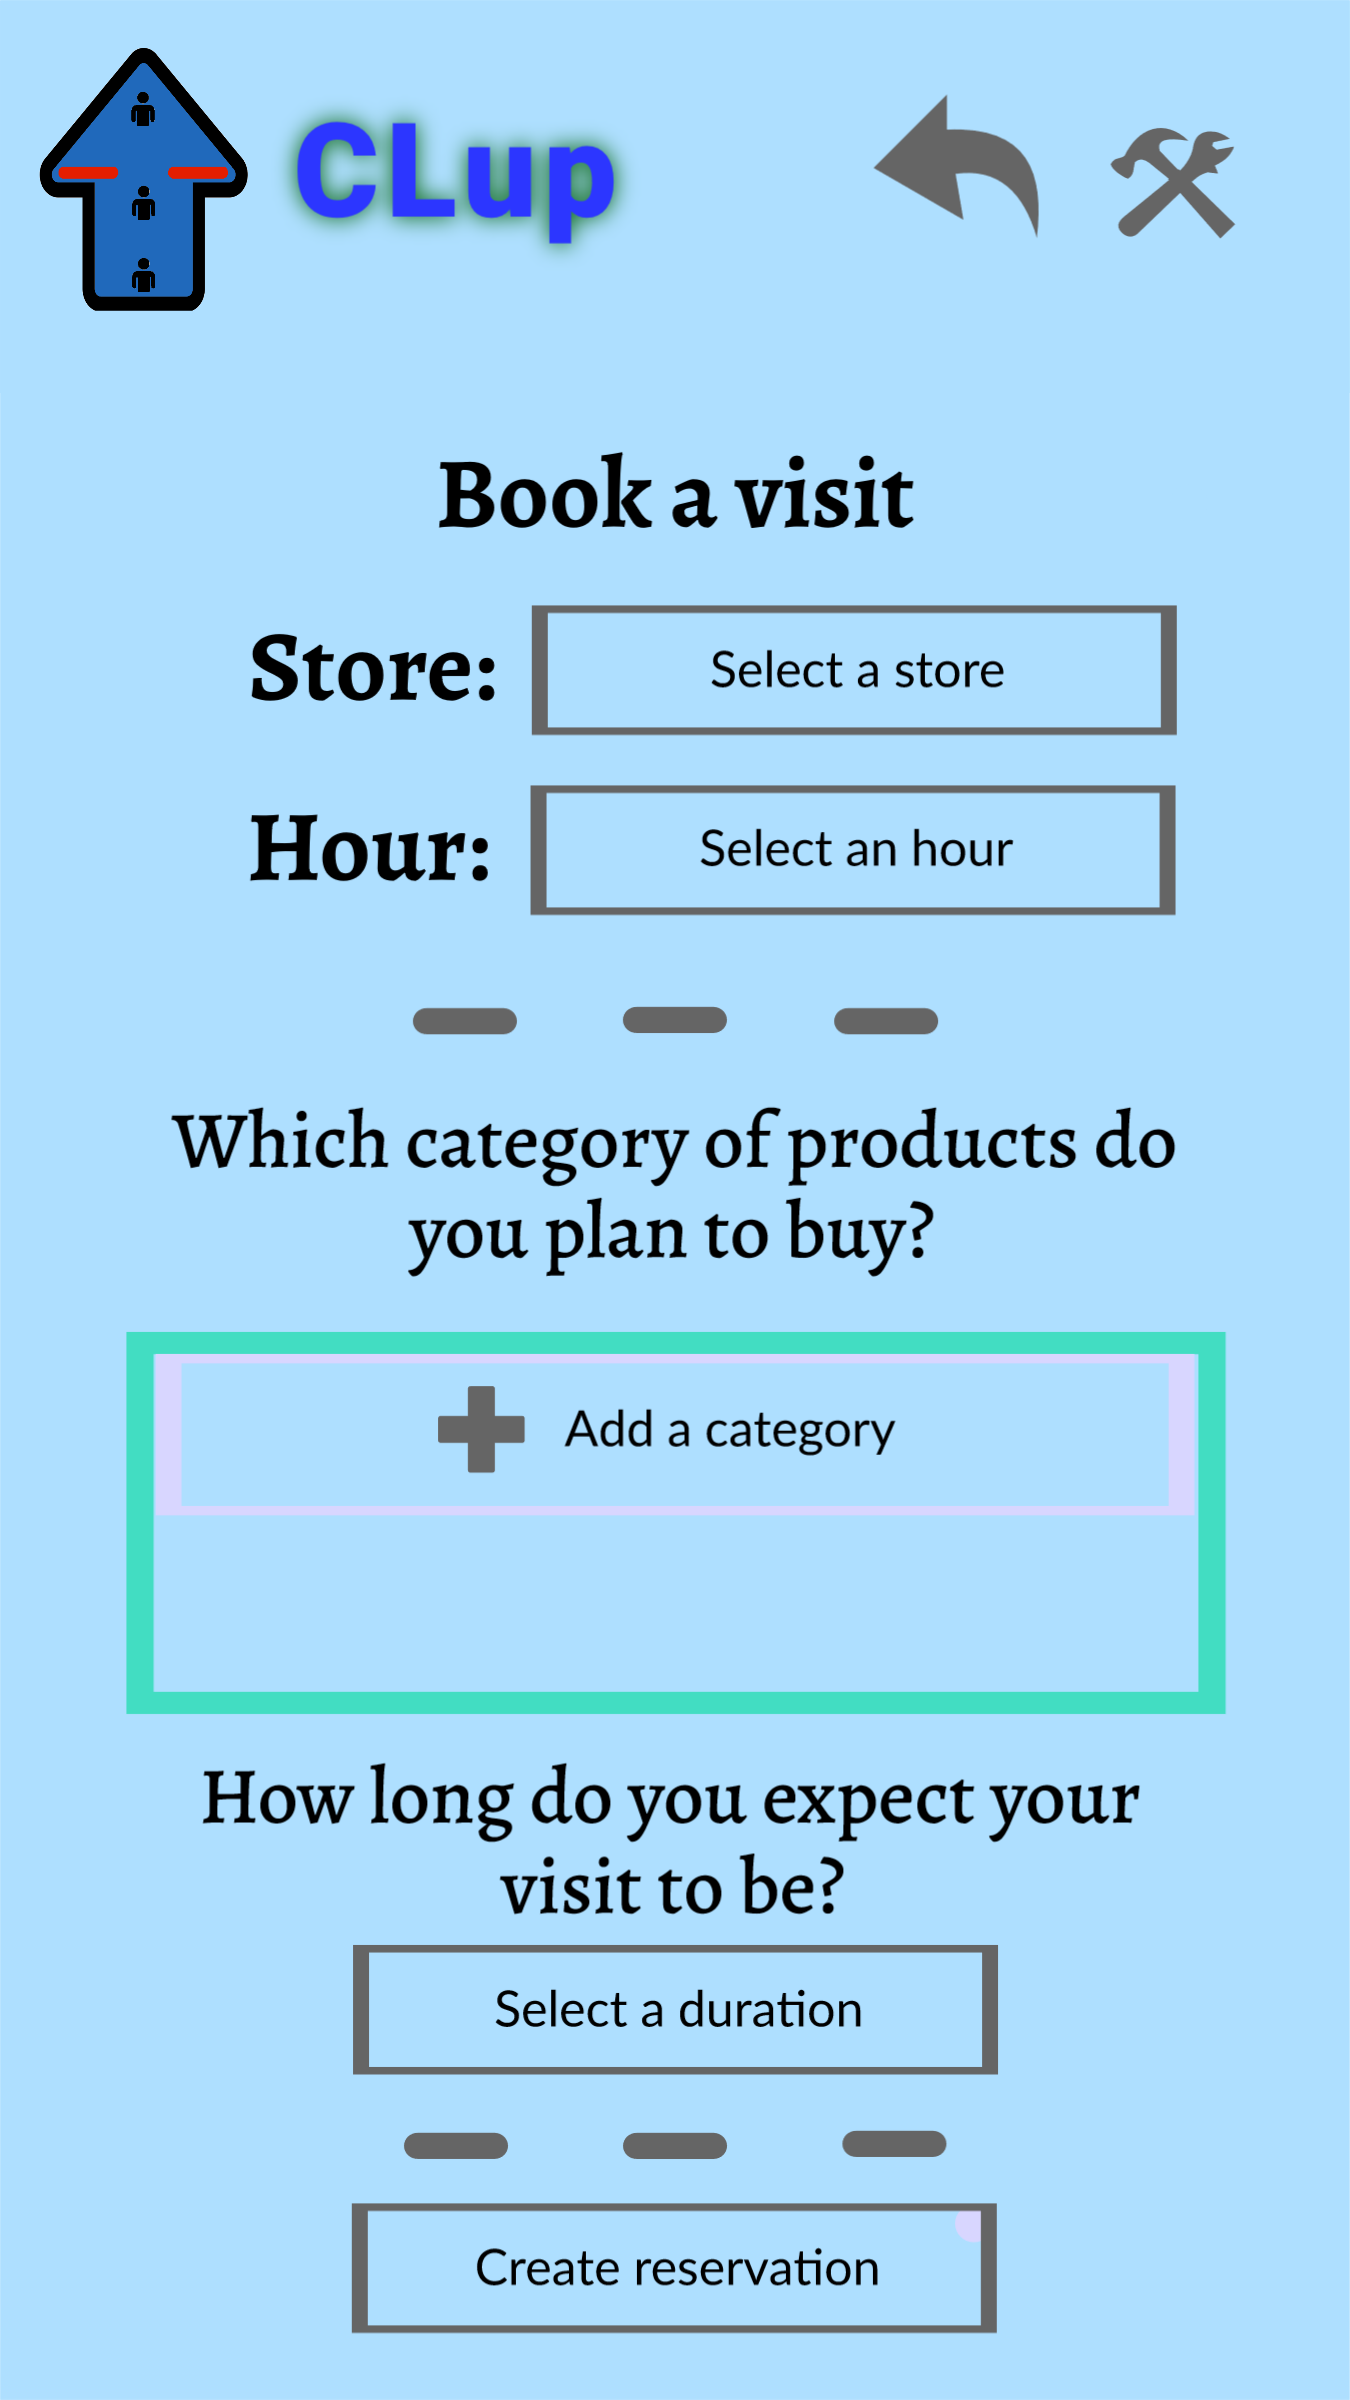
\includegraphics[scale=0.1]{Images/BookAVisit.png}
	%TODO add by car/on foot icons
	\qquad
	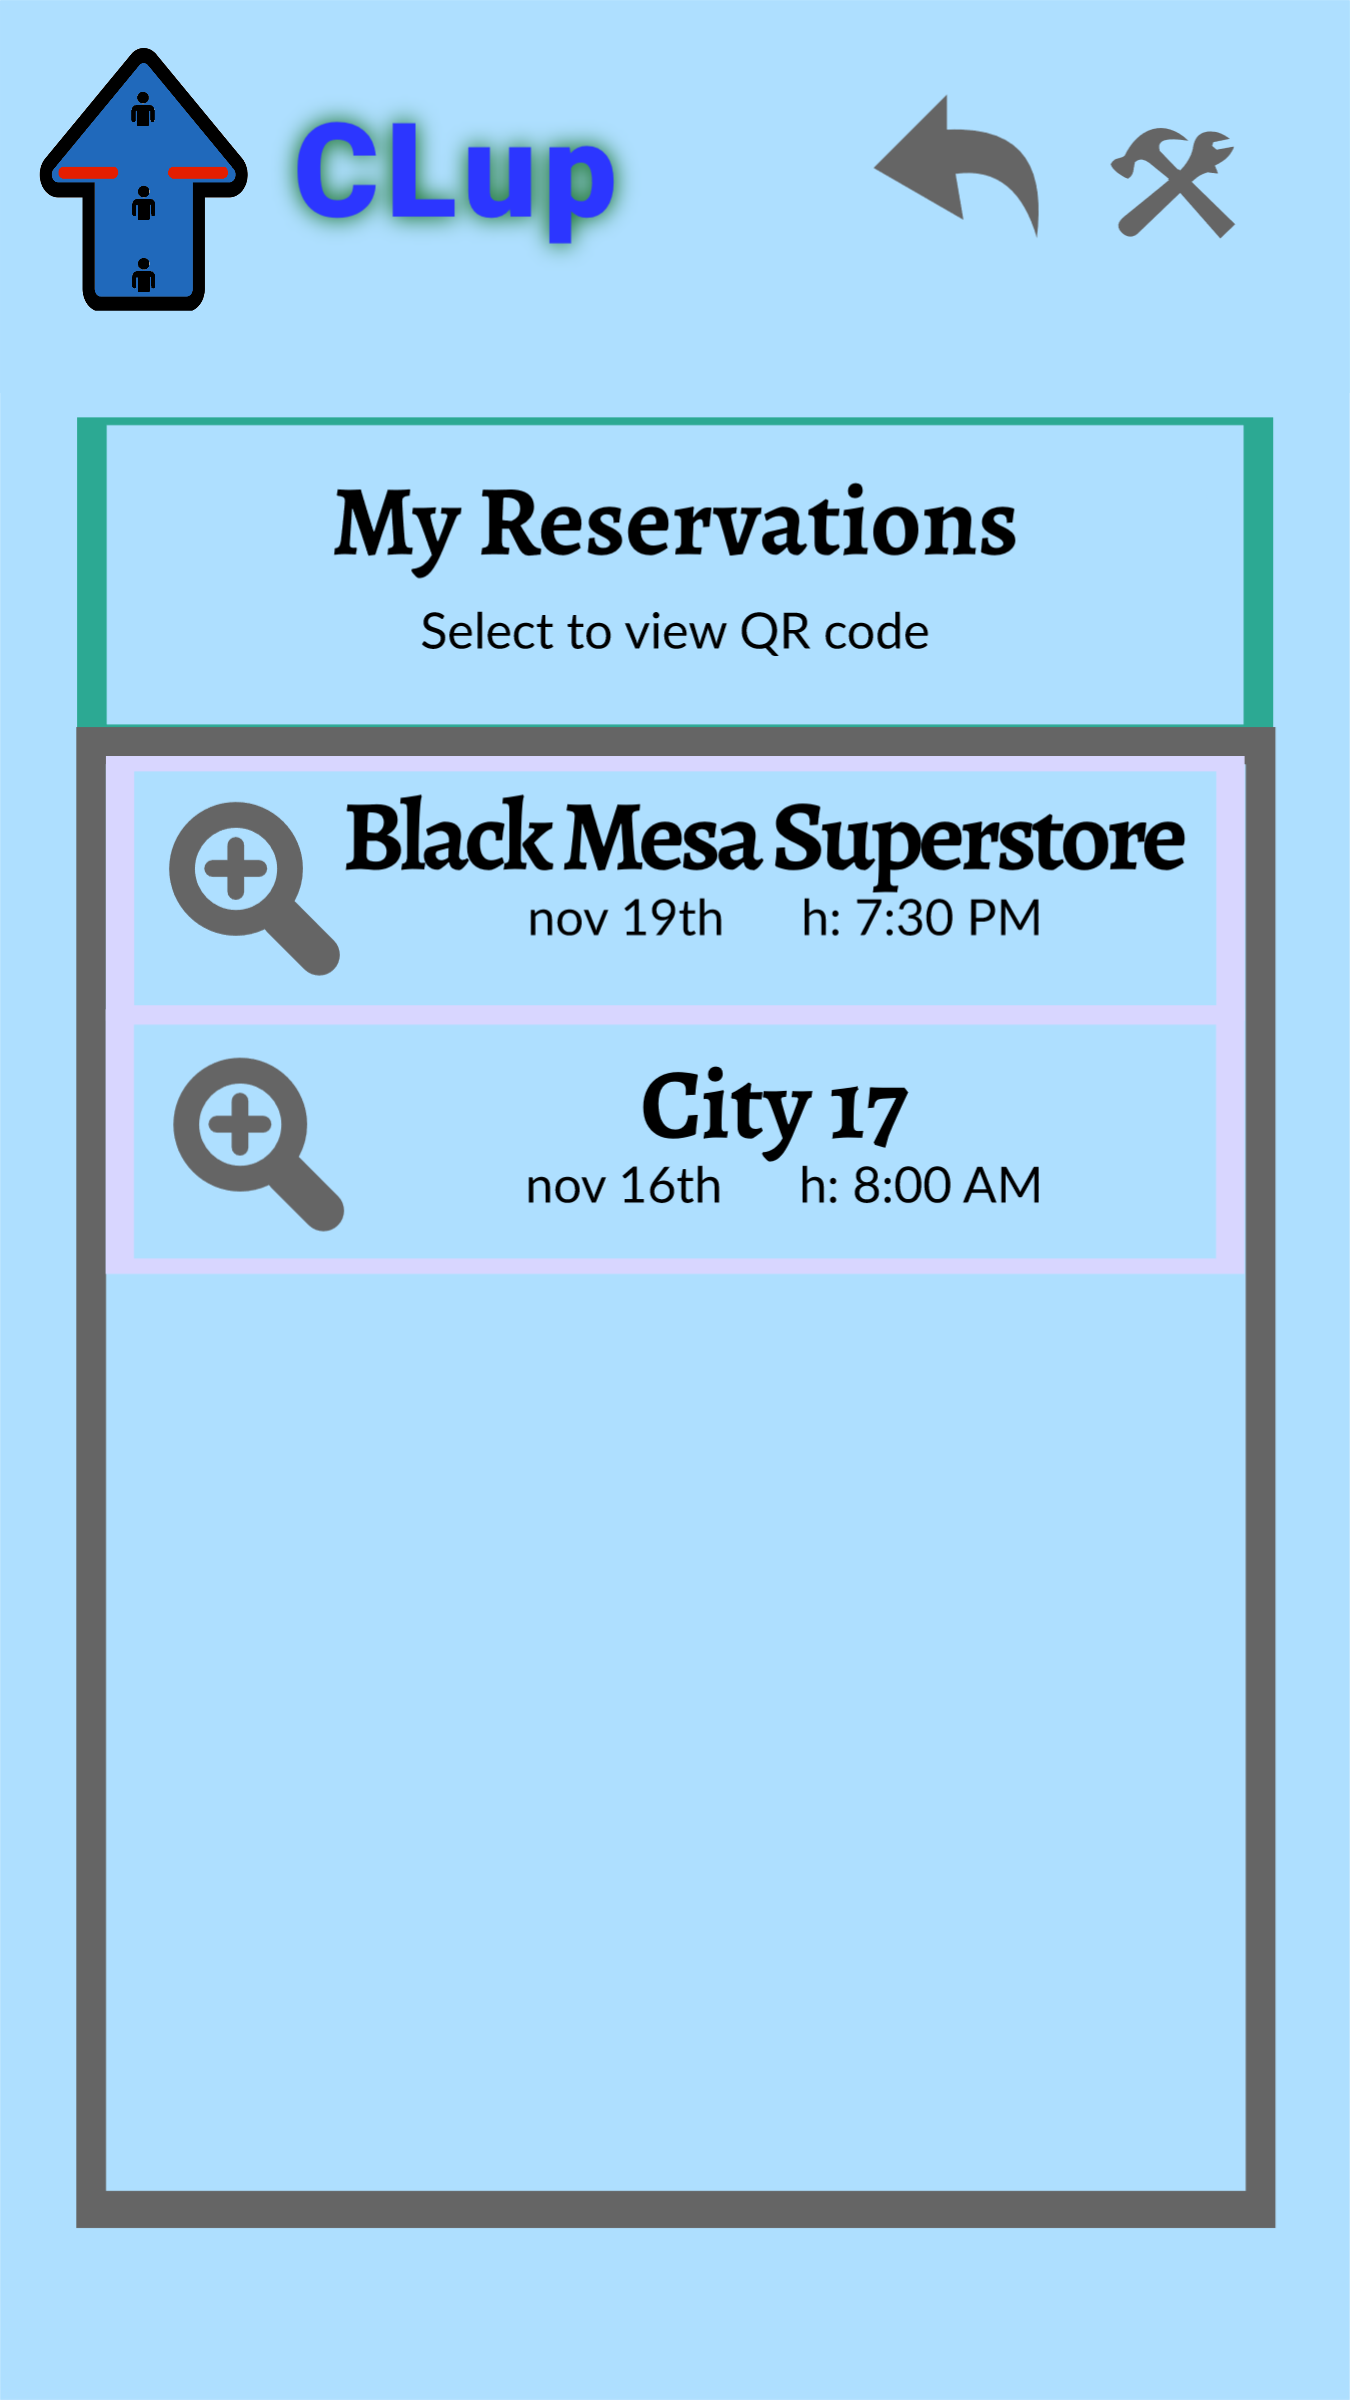
\includegraphics[scale=0.1]{Images/ShowReservations.png}
	\item {\bfseries Store owners}\\
	The store owner is presented with a main menu from which he/she can:
		\begin{itemize}
		\item register a store to the system
		\item delete a store from the system
		\item view and edit occupation for currently registered stores
	\end{itemize}
	\begin{figure}[!htb]
		\centering
		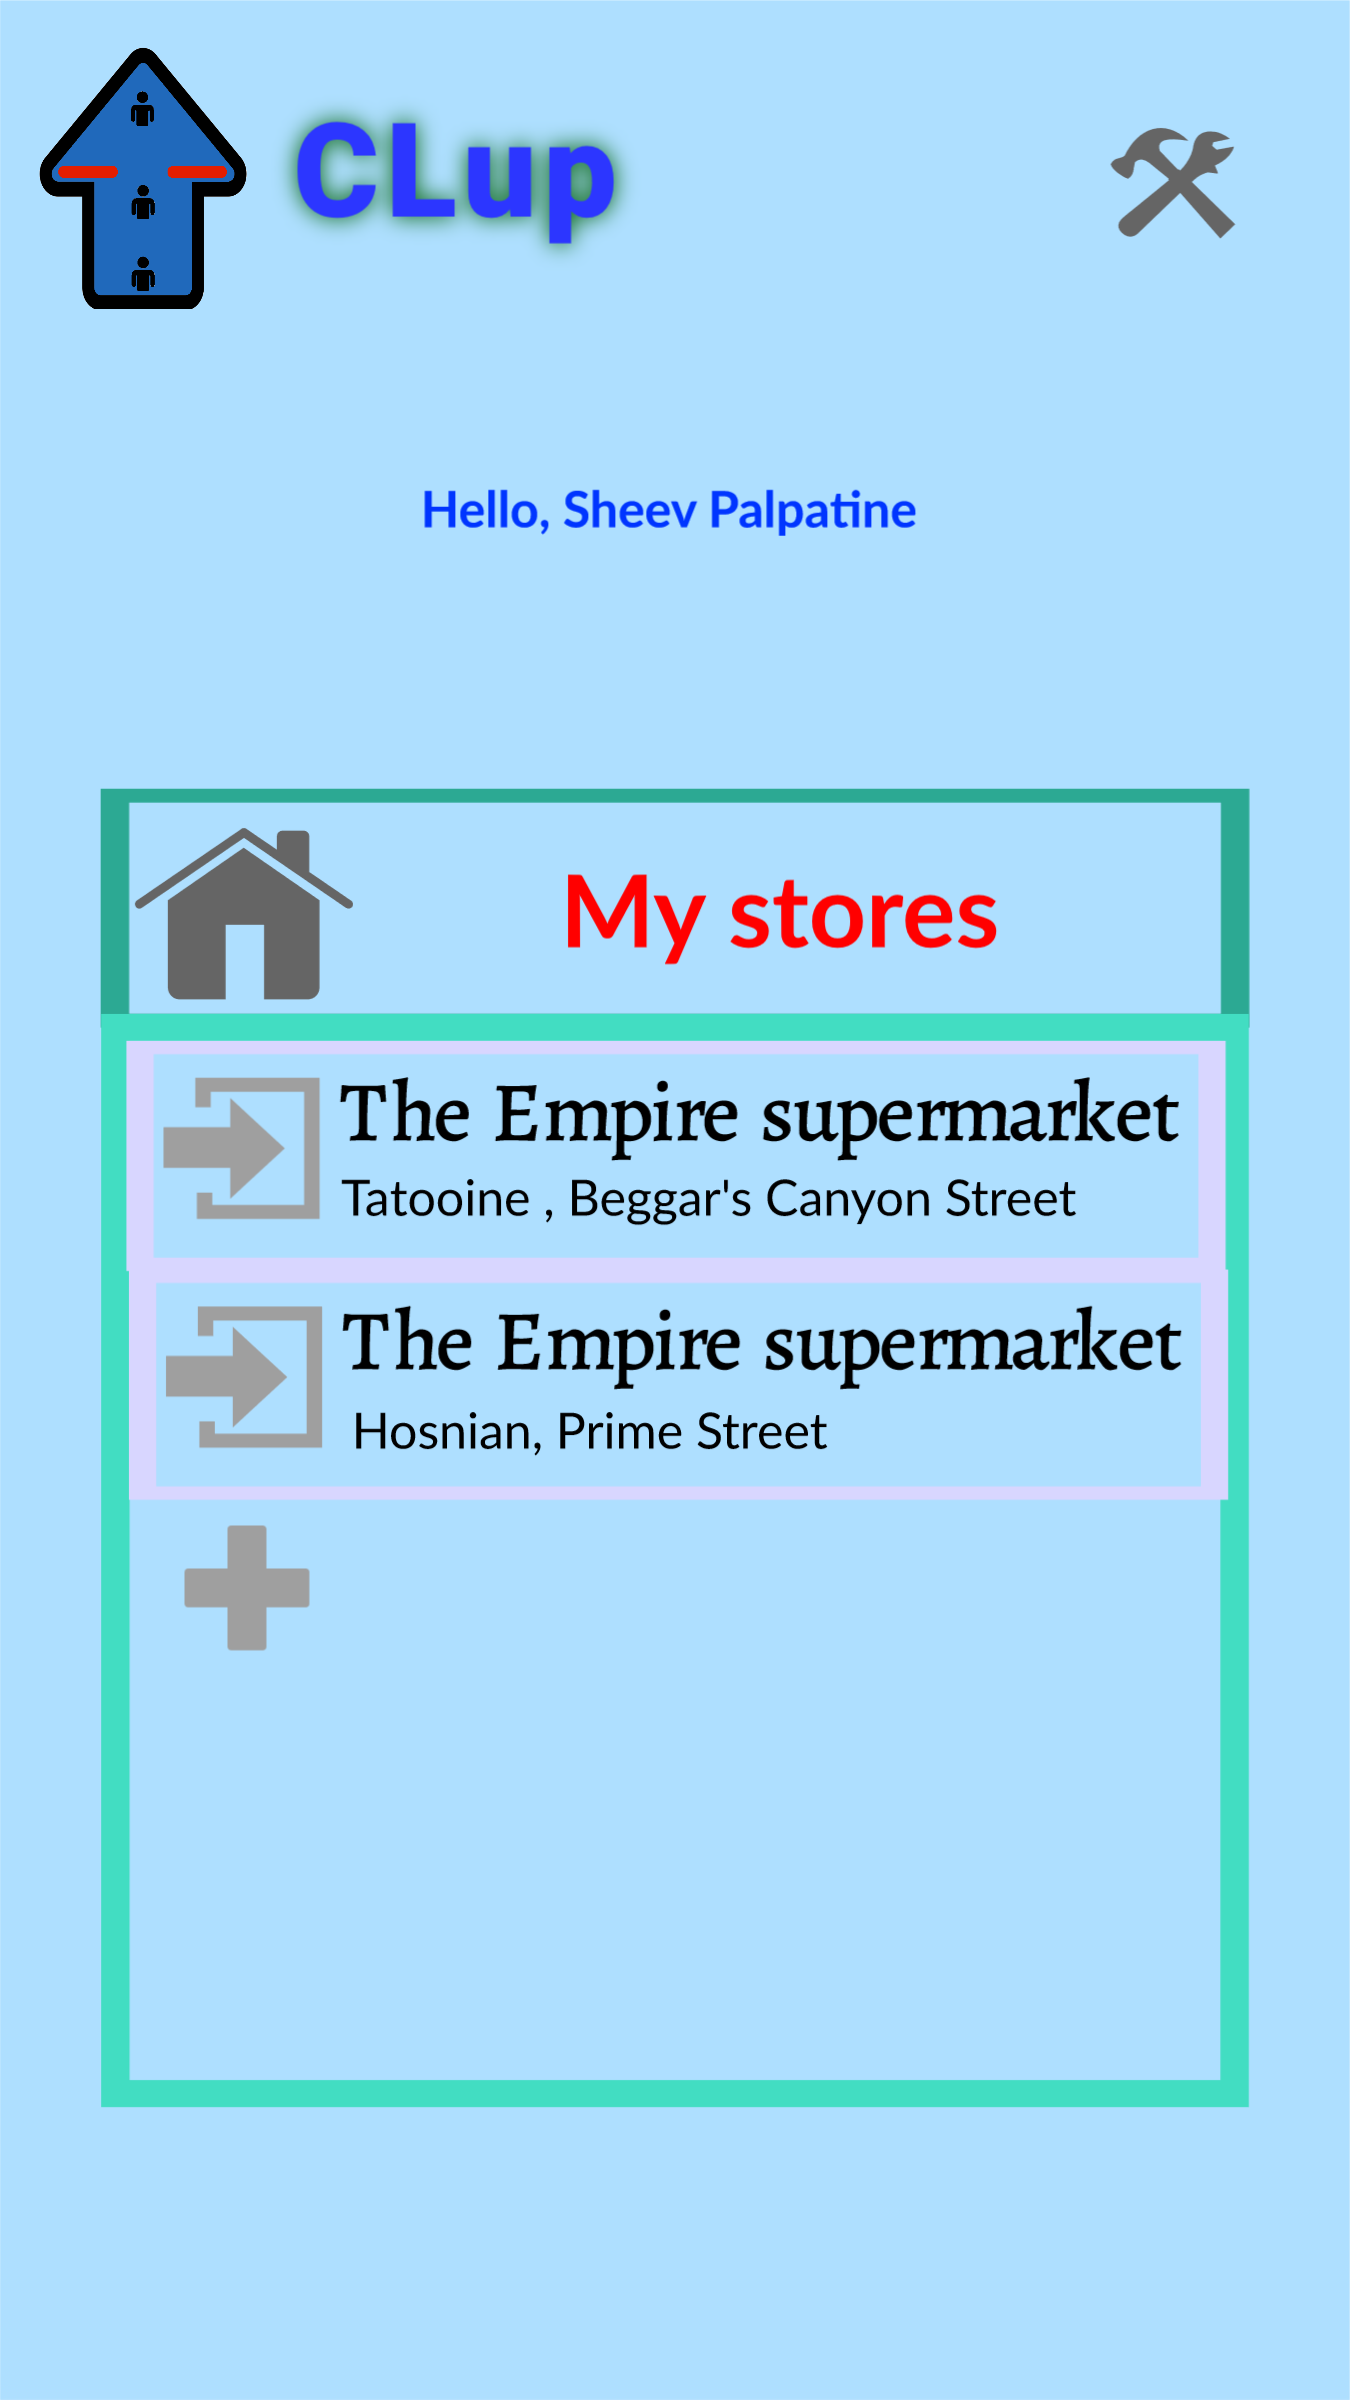
\includegraphics[scale=0.1]{Images/MainMenuOwner.png}
		\qquad \qquad
		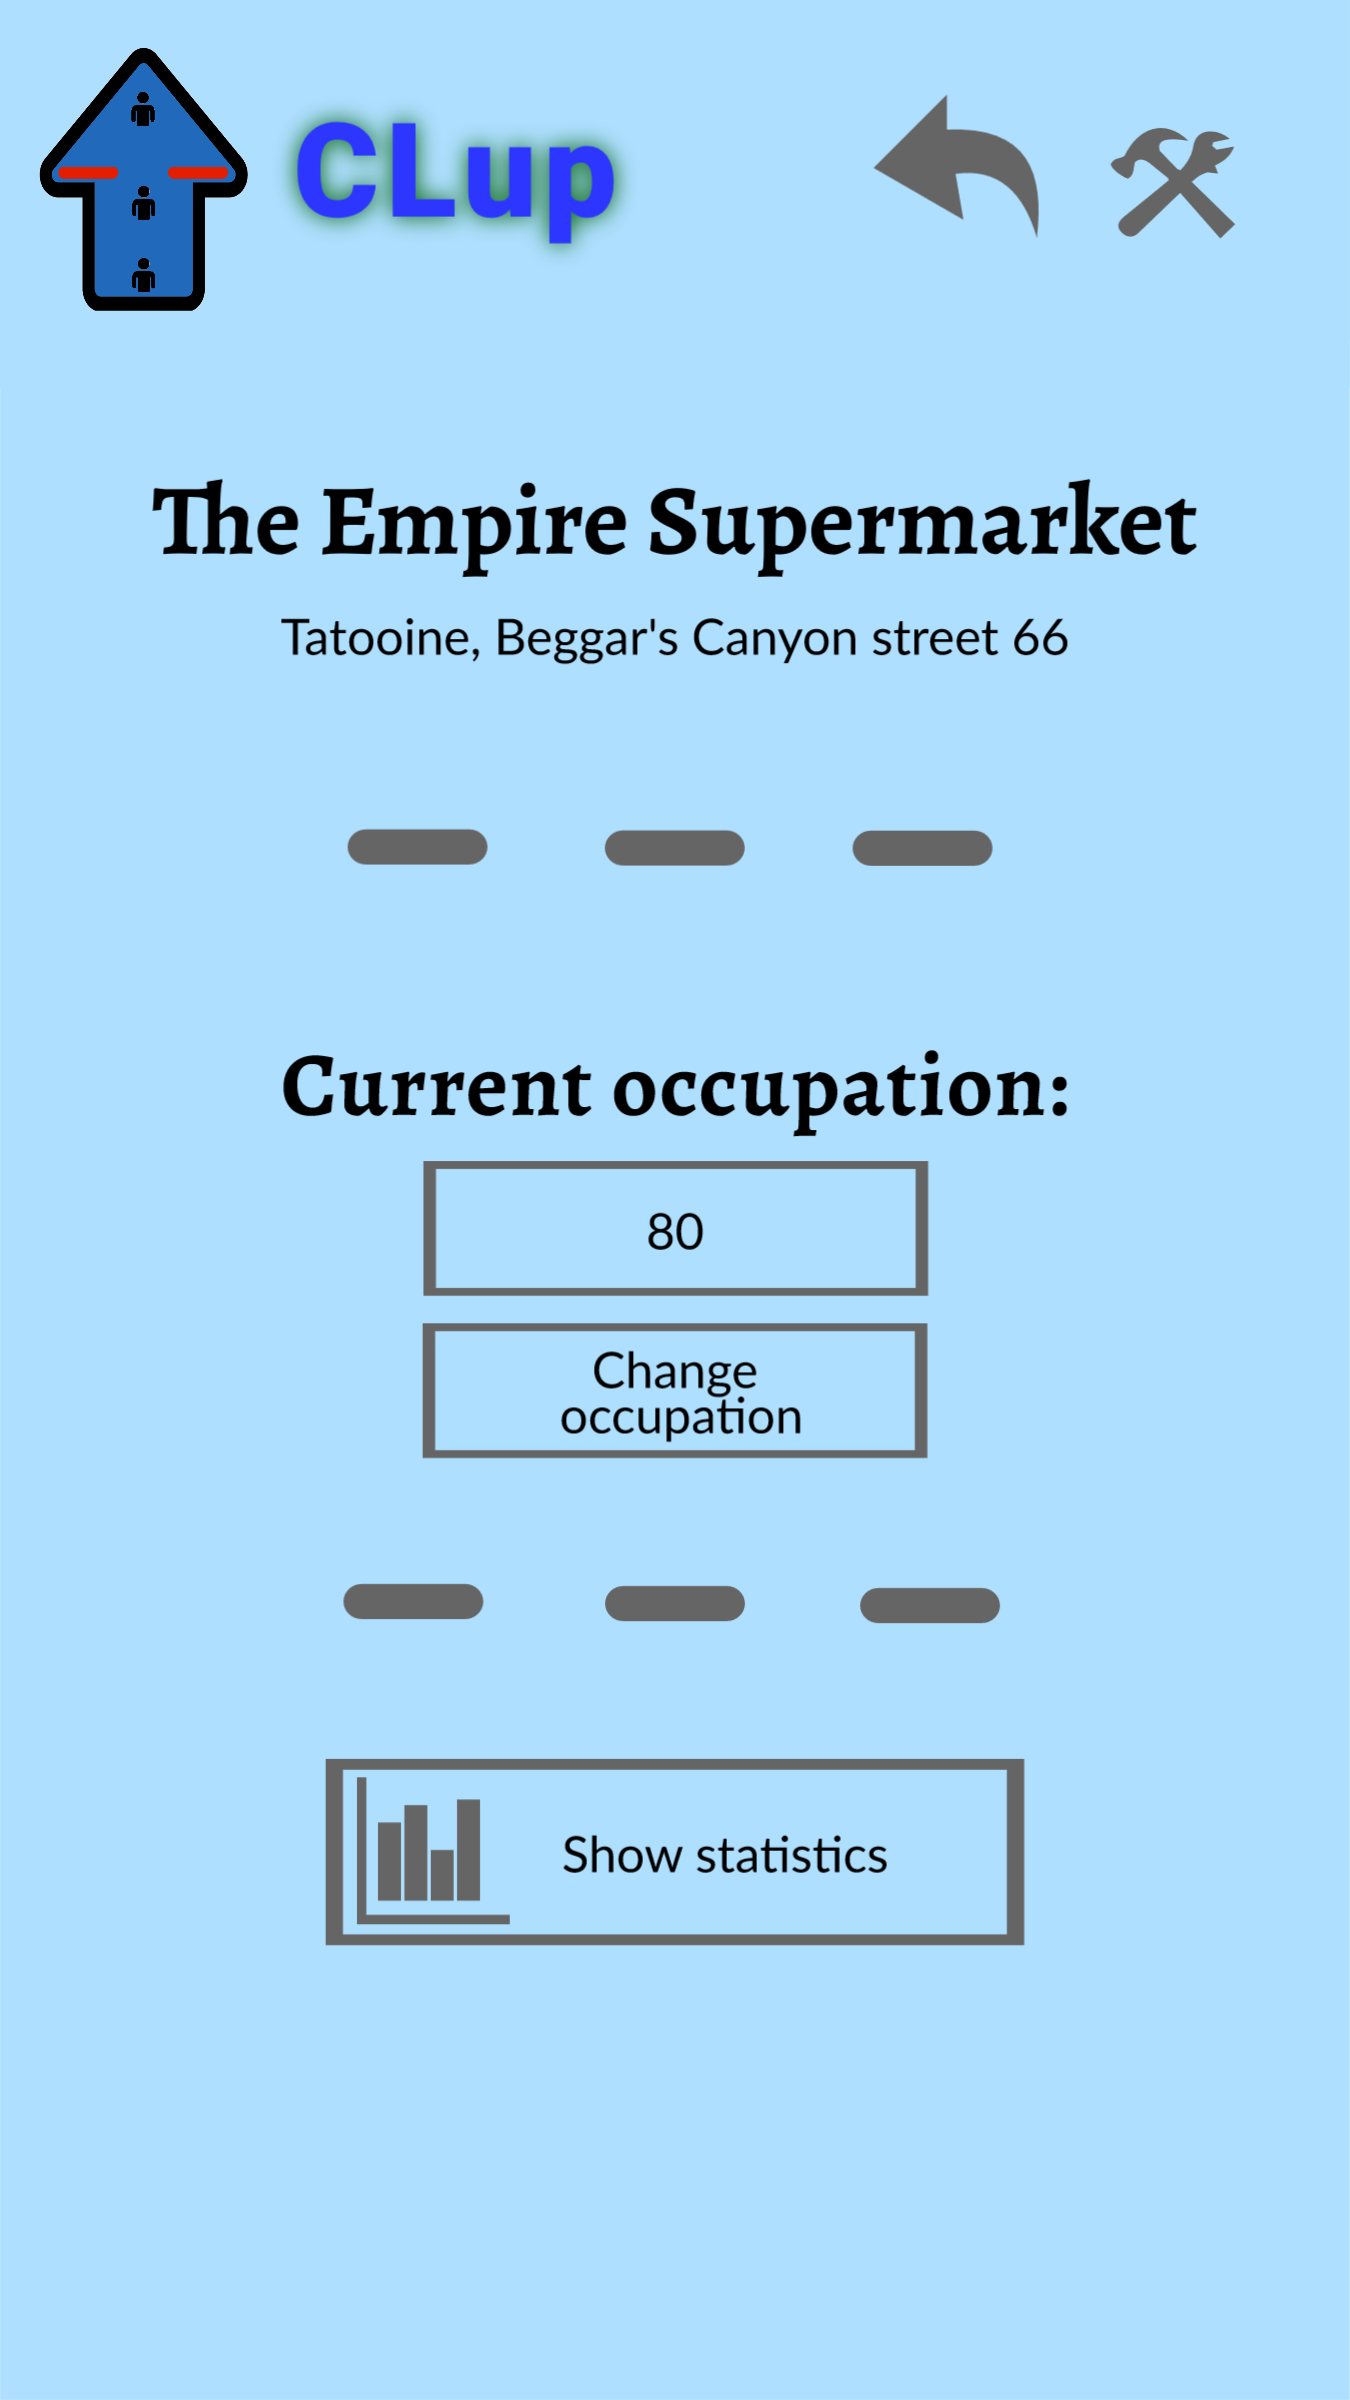
\includegraphics[scale=0.1]{Images/ModifyOccupation.png}
	\end{figure}
	
\end{itemize}
\subsubsection{Hardware interfaces}
The S2B requires the following hardware interfaces:
\begin{enumerate}
	\item {\bfseries Computer or smartphone}\\
	Users will need a computer or a smartphone to access the system's services which are provided via an application (only for smartphone owners) and a web application. Only users with an application will be able to receive notifications that alert them when it is time for them to depart and reach the store.
	\item {\bfseries Turnstiles}\\
	Turnstiles allow authorized customers to enter or exit the store by providing a means of identification. (i.e. QR, NFC)
	\item {\bfseries Ticket printer}\\
	The ticket printers located outside stores allows potential customers to queue up on premise provided that they identify themselves (e.g. social security card).
	\item \textbf{Monitor}\\
	A monitor located outside stores allows customers that queue up on premise to know when it is time for them to access the store.
\end{enumerate}

\subsubsection{Software interfaces}
The system uses a public API to locate the customer and provide him/her with notifications about the time he will need to depart to reach the store.

\subsubsection{Communication interfaces}
Customers can access the system through a working internet connection.

\subsection{Functional requirements}
\subsubsection{List of requirements}
\begin{enumerate}[label=R\arabic*]
	\item Turnstiles unlock if and only if activated by authorized customers.
	\item The number of customers in each department of the store never exceeds the occupation set by the owner.
	\item The monitor outside the store displays the number of the last authorized customer.
	\item The system allows customers and store owners to register and log in.
	\item The system validates the authenticity of the identifying information provided.
	\item The system allows customers to search for a store among those registered by their owners.
	\item Registered customers can send a reservation request to the system.
	\item Non registered customers with an identifying document can request reservations through the printer.
	\item Registered customers that book a visit can specify estimated visit duration.
	\item Registered customers that book a visit can specify desired product categories.
	\item The system provides customers with a QR code to enter the store once authorized.
	\item The system uses gathered data to build statistics. %TODO to ask.
	\item Registered customers with a smartphone are alerted when their turn is near.

	\item Registered customers can delete a pending or authorized reservation.
	\item After a reservation is authorized if it does not become current in a fixed time, it expires.
	\item Registered customers must specify desired means of transport while requesting a reservation.
	\item Reservations are authorized according to a FIFO policy 

	%TODO add that customers have a time window in which they can enter a store after which their reservation expires, otherwise the store could remain empty (limit case)
	
	%TODO pensare a come sistemare la faccenda dell'occupazione dei dipartimanti/massima
\end{enumerate}
\subsubsection{Mapping on requirements}
\begin{tabular}{ | m{3cm} | m{5cm} | m{9cm} | }
	\hline
	G1 & D1, D2, D5, D6, D8, D9 & R1, R2, R4, R5, R6, R7, R11, R16, R17\\
	\hline
	G2 & D1, D2, D3, D4, D5, D6 & R1, R2, R3, R5, R8, R11, R17\\
	\hline
	G3 & D1, D2, D3, D4, D5, D6, D8, D9 & R1, R2, R3, R4, R5, R6, R7, R9, R10, R11, R16, R17\\
	\hline
	G4 & D1, D2, D5, D8, D9 & R1, R2 \\
	\hline
	G5 & D8, D9 & R9, R12, R14, R15\\
	\hline
	G6 & D7, D8, D9 & R13\\
	\hline

\end{tabular}
\begin{enumerate}[label=G\arabic*]
	\item CLup should allow customers to queue up remotely
	\item CLup should allow customers to queue up on premise
	\item CLup should allow customers to book future visits to stores
	\item CLup should allow store owners to regulate the maximum number of customers in their stores
	\item CLup should provide the customer with a reasonably precise estimate of waiting time
	\item CLup should alert the customers when it is time to get to the shop taking into account travel time
	%\item CLup should allow customers to specify estimated visit duration and desired objects in order to provide a better guess of waiting time for all the customers
	%TODO is this a goal or a reqirement???
	% CLup should be able to infer an approximate duration of the visit from an analysis of the previous ones to plan visits and manage the queue in a finer way
\end{enumerate}
\begin{enumerate}[label=D\arabic*]
	\item The stores have QR activated turnstiles.
	\item Turnstiles let one and only one person in each time they unlock.
	\item Outside stores is a social security card activated ticket printer.
	\item Outside stores there is a monitor.
	\item There is no way for a customer to enter a store except from entrance and exit.
	\item Each customer has either a telephone number or an identification document.
	\item When provided, user location has maximum error of 5 meters.
	\item To register to the S2B users must have either a smartphone or a computer.
	\item To register and use the S2B users must have an internet connection.
\end{enumerate}
\subsubsection{Use case diagram}
\subsubsection{Use cases}
%TODO: 'customer is notified' use case: is it useless?
\paragraph{Customer registration}
\begin{flushleft}
	\begin{tabular} { | m{3cm} | m{10cm} | }
		\hline
		Name & Customer registration\\
		\hline
		Actors & Customer\\
		\hline
		Entry condition & Customer has opened the smartphone application or the web app on his computer but has not logged in\\
		\hline
		Event flow & \begin{enumerate}
			\item a registration menu is provided to the customer
			\item from such menu the customer selects the option to sign up as customer
			\item the customer is then prompted to insert identifying information
			\item the customer inserts requested information
			\item the system validates provided information
			\item the system confirms the registration of the customer and saves information provided
		\end{enumerate}\\
		\hline
		Exit conditions & Customer has registered to the system\\
		\hline
		Exceptions & \begin{enumerate}
			\item a customer with same identifying information already exists
			\item validation of identifying information is not successful
			\item the customer decides to cancel the registration
		\end{enumerate}
		If one of the first two events described above occur, the application will alert the customer and provide him with the possibility to retry or go back to the initial menu.\newline If event 3 occurs the customer is redirected to the main page.\\
		\hline
	\end{tabular}
\end{flushleft}

\paragraph{Store owner registration}
\begin{flushleft}
	\begin{tabular} { | m{3cm} | m{10cm} | }
		\hline
		Name & Store owner registration\\
		\hline
		Actors & Store owner\\
		\hline
		Entry condition & Store owner has opened the smartphone application or the web app on his computer but has not logged in\\
		\hline
		Event flow & \begin{enumerate}
			\item a registration menu is provided to the store owner
			\item from such menu the store owner selects the option to sign up as store owner
			\item the store owner is then prompted to insert identifying information
			\item the store owner inserts requested information
			\item the system validates provided information
			\item the system confirms the registration of the store owner and saves information provided
		\end{enumerate}\\
		\hline
		Exit conditions & Store owner has registered to the system\\
		\hline
		Exceptions & \begin{enumerate}
			\item a store owner with same identifying information already exists
			\item validation of identifying information is not successful
			\item the store owner decides to cancel the registration
		\end{enumerate}
		If one of the first two events described above occur, the application will alert the store owner and provide him with the possibility to retry or go back to the initial menu.\newline If event 3 occurs the store owner is redirected to the main page.\\
		\hline
	\end{tabular}
\end{flushleft}

\paragraph{User logs in}
\begin{flushleft}
	\begin{tabular} { | m{3cm} | m{10cm} | }
		\hline
		Name & User logs in\\
		\hline
		Actors & Customer or store owner\\
		\hline
		Entry condition & The user has opened the application on his device, and has already registered to the system\\
		\hline
		Event flow & \begin{enumerate}
            \item User chooses to log in from the welcome menu
            \item User identifies him/herself with created credentials
		\end{enumerate}\\
		\hline
		Exit conditions & User is logged in\\
		\hline
		Exceptions & \begin{enumerate}
			\item User credentials are invalid
		\end{enumerate}
		%TODO store e chiuso
		If the event described above occurs, the application will alert the user and allows him to retry\\
		\hline
	\end{tabular}
\end{flushleft}

\paragraph{Customer queuing up remotely}
\begin{flushleft}
	\begin{tabular} { | m{3cm} | m{10cm} | }
		\hline
		Name & Customer queuing up remotely\\
		\hline
		Actors & Customer\\
		\hline
		Entry condition & Customer has logged in on the smartphone application or the web app on his computer\\
		\hline
		Event flow & \begin{enumerate}
			\item customer selects to queue up from main menu
			\begin{itemize}
				\item with an immediate reservation
				\item with a future reservation (and optionally inserts desired categories of item he/she intends to buy and how much time he/she intends to spend at the store)
			\end{itemize}
			\item customer selects a store from the list of stores registered to the system
			\item customer specify  whether he is going to reach the store by car or on foot
			\item customer submits reservation request
		\end{enumerate}\\
		\hline
		Exit conditions & Customer reservation is confirmed\\
		\hline
		Exceptions & \begin{enumerate}
			\item customer decides to cancel the reservation
			\item customer requests immediate reservaiton but store is closed at that time
		\end{enumerate}
	%TODO store e chiuso
		If one of the events described above occur, the application will alert the customer and go back to the initial menu\\
		\hline
	\end{tabular}
\end{flushleft}

\paragraph{Customer queuing up on premise}
\begin{flushleft}
	\begin{tabular} { | m{3cm} | m{10cm} | }
		\hline
		Name & Customer queuing on premise\\
		\hline
		Actors & Customer\\
		\hline
		Entry condition & Customer has reached the store ticket printer\\
		\hline
		Event flow & \begin{enumerate}
			\item customer selects the option to queue up from main menu of the ticket printer
			\item customer provides the ticket printer with a means of identification (e.g. social security card)
		\end{enumerate}\\
		\hline
		Exit conditions & Customer reservation is confirmed and a ticket is printed containing the following information:
		\begin{itemize}
			\item how much time he needs to wait before being able to enter the store
			\item a progressive number that will allow him to know when his/her turn is
		\end{itemize}\\
		\hline
		Exceptions & \begin{enumerate}
			\item customer decides to cancel the reservation
		\end{enumerate}
		If one of the events described above occur, the application will alert the customer and go back to the initial menu\\
		\hline
	\end{tabular}
\end{flushleft}

\paragraph{Customer entering store}
\begin{flushleft}
	\begin{tabular} { | m{3cm} | m{10cm} | }
		\hline
		Name & Customer entering store\\
		\hline
		Actors & Customer\\
		\hline
		Entry condition & Customer has logged in on the smartphone application and is at the entrance of a store or has printed authorization from the web app\\
		\hline
		Event flow &
		If the customer has not printed the reservation ticket he must use his smartphone:
		\begin{enumerate}
			\item customer selects the option to show existing reservations from main menu of the phone app 
			\item customer selects an existing reservation and if authorized (i.e. it is his turn to enter the store) he/she is given the means to identify him/herself (e.g. display QR or activate NFC)
		\end{enumerate}
		Then the customer identifies him/herself at the turnstiles\\
		\hline
		Exit conditions & Customer enters the store\\
		\hline
		Exceptions & \begin{enumerate}
			\item customer is not authorized to enter the store
		\end{enumerate}
		If the event described above occurs, the turnstiles will not let the customer in\\
		\hline
	\end{tabular}
\end{flushleft}

\paragraph{Customer exiting store}
\begin{flushleft}
	\begin{tabular} { | m{3cm} | m{10cm} | }
		\hline
		Name & Customer exiting store\\
		\hline
		Actors & Customer\\
		\hline
		Entry condition & Customer has logged in on the smartphone application and is in a store\\
		\hline
		Event flow &
		If the customer has not printed the reservation ticket he must use his smartphone:
		\begin{enumerate}
			\item customer selects the option to show existing reservations from main menu
			\item customer selects an existing reservation and if authorized (i.e. it is his turn to enter the store) he/she is given the means to identify him/herself (e.g. display QR or activate NFC)
		\end{enumerate}
	    Customer identifies him/herself at the turnstiles\\
		\hline
		Exit conditions & Customer exits the store\\
		\hline
		Exceptions & \\
		\hline
	\end{tabular}
\end{flushleft}

\paragraph{Store owner registering a store}
\begin{flushleft}
	\begin{tabular} { | m{3cm} | m{10cm} | }
		\hline
		Name & Store owner registering a store\\
		\hline
		Actors & Store owner\\
		\hline
		Entry condition & Store owner has logged in on the smartphone application or the web app on his computer\\
		\hline
		Event flow & \begin{enumerate}
			\item store owner selects the option register a store from main menu
			\item store owner inserts necessary information and sets up equipment (i.e. connect printer, monitor and turnstiles to the system)
			\item store owner submits store registration request
		\end{enumerate}\\
		\hline
		Exit conditions & Store registration is confirmed\\
		\hline
		Exceptions & \begin{enumerate}
			\item information is missing or incorrect
			\item equipment is not working properly			\item store owner decides to cancel the store registration
		\end{enumerate}
		If one of the events described above occur, the application will alert the store owner and provide him with the possibility to retry or go back to the initial menu\\
		\hline
	\end{tabular}
\end{flushleft}

\paragraph{Store owner setting maximum occupation of one of his stores}
\begin{flushleft}
	\begin{tabular} { | m{3cm} | m{10cm} | }
		\hline
		Name & Store owner setting maximum occupation of one of his stores\\
		\hline
		Actors & Store owner\\
		\hline
		Entry condition & Store owner has logged in on the smartphone application or the web app on his computer\\
		\hline
		Event flow & \begin{enumerate}
			\item store owner selects one of his stores from the list reachable form the main menu
			\item store owner views current occupation of his store, and current occupation threshold
			\item sets the new desired occupation threshold
		\end{enumerate}\\
		\hline
		Exit conditions & The new occupation threshold is set\\
		\hline
		Exceptions & \begin{enumerate}
			\item the threshold value is inadequate
		\end{enumerate}
		If the event described above occurs, the application will alert the store owner and provide him with the possibility to retry or go back to the initial menu\\
		\hline
	\end{tabular}
\end{flushleft}
\subsubsection{Sequence diagrams}
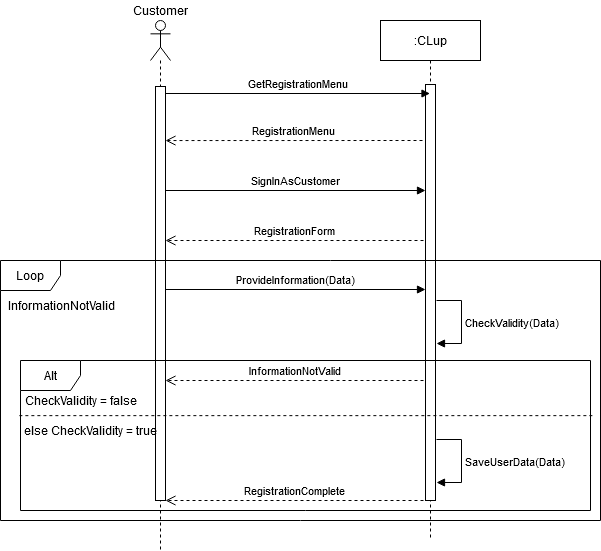
\includegraphics[scale=0.5]{Images/UseCase1Diagram.png}\\\\
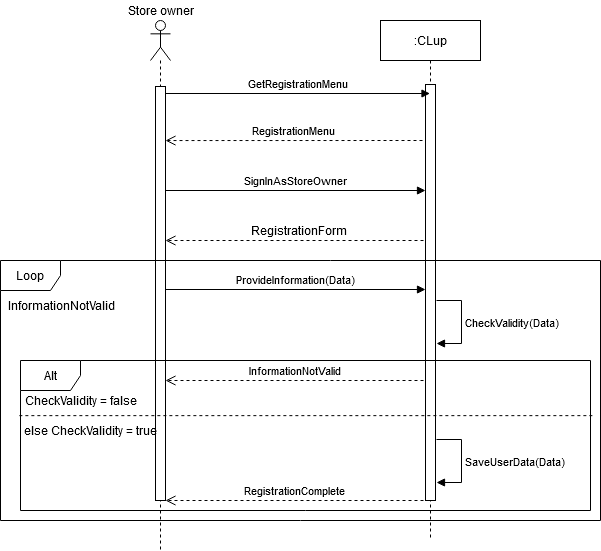
\includegraphics[scale=0.5]{Images/UseCase2Diagram.png}\\\\
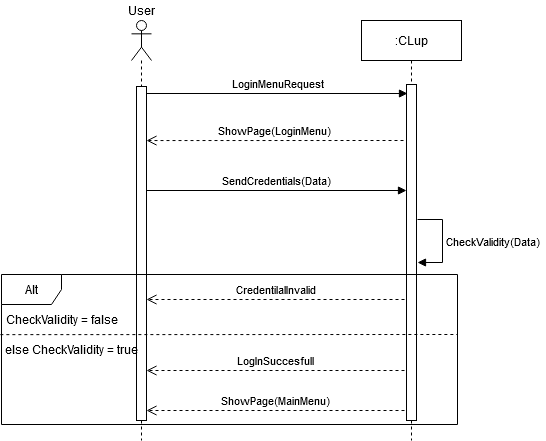
\includegraphics[scale=0.5]{Images/UseCase3Diagram.png}\\\\
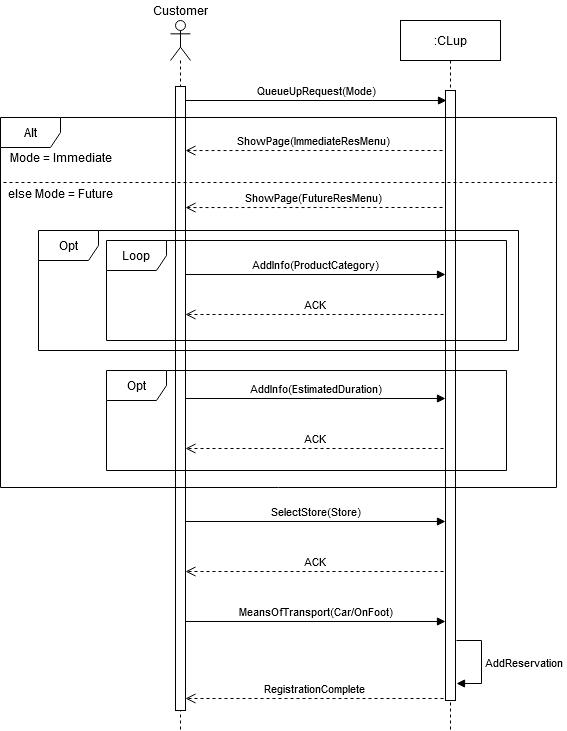
\includegraphics[scale=0.5]{Images/UseCase4Diagram.png}\\\\
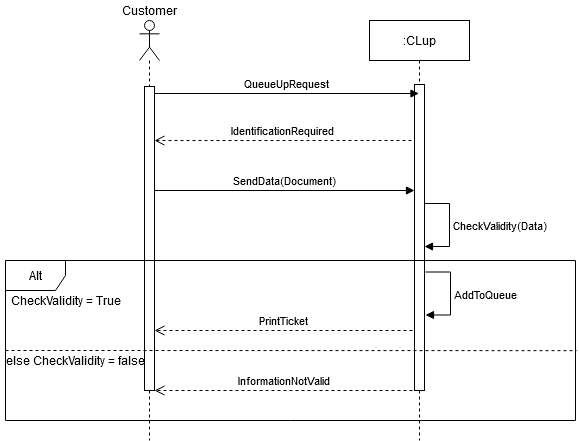
\includegraphics[scale=0.5]{Images/UseCase5Diagram.png}\\\\
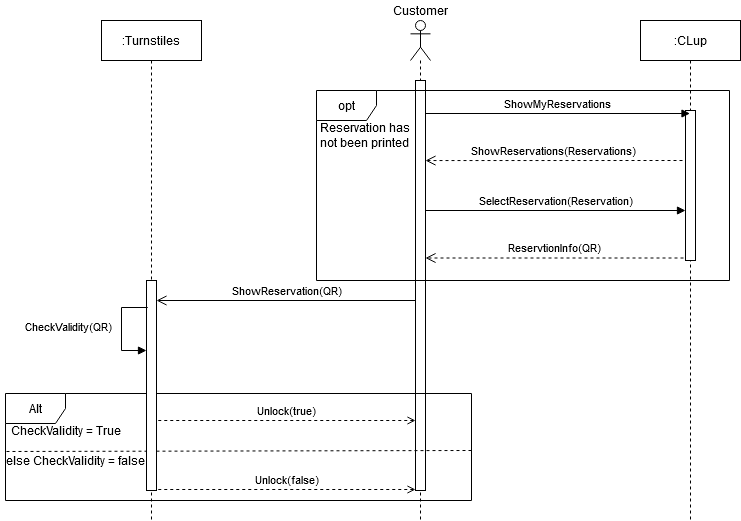
\includegraphics[scale=0.5]{Images/UseCase6-7Diagram.png}\\\\
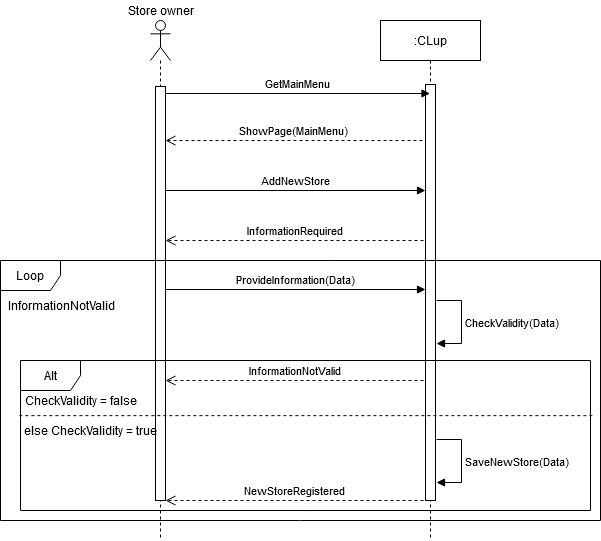
\includegraphics[scale=0.5]{Images/UseCase8Diagram.png}\\\\
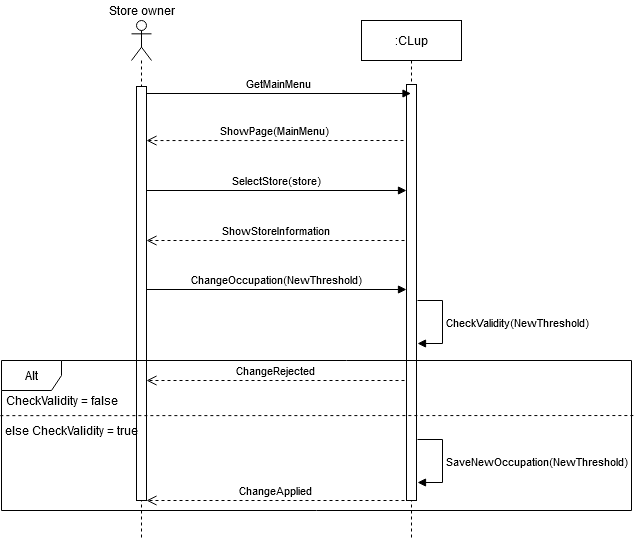
\includegraphics[scale=0.5]{Images/UseCase9Diagram.png}\\\\
\subsubsection{Scenarios} %TODO: should they go to section 2 as assignment says?
\paragraph{Customer queues up remotely}
Gordon comes home from work at 5:30 PM. He would like to go to the store. He is a registered user of CLup. His smartphone has internet connection and GPS on. He opens the CLup mobile application and requests an immediate reservation to a store of his choice, selecting the car as means of transport. After some time he is alerted that he needs to depart to avoid being late at the store and losing the reservation. Pietro departs and arrives to the store. He opens the application and selects the reservation he created which now contains the number that represents his position in the queue. After some time the monitor outside the store shows his number, which means it is his turn to enter. He activates the turnstiles with the QR now shown in the reservation page of the mobile application and enters the store. He buys all the products he needs. He opens the application and selects the reservation he created which now contains a QR code. He activates the turnstiles and exits the store.
%TODO: be like Pietro
\paragraph{Customer queues up on premise}
Marco is an old man. He does not have a smartphone. He would like to go to the store next to his house on foot. He reaches the store, and retrieves a queue reservation ticket from the printer outside the store, by inserting his social security card. The ticket displays a QR code and a number that represents his position in queue. After some time the monitor outside the store shows his number, which means it is his turn to enter. He activates the turnstiles with the QR printed on his ticket and enters the store. He buys all the products he needs. He activates the turnstiles with his ticket and exits the store.
\subsection{Performance Requirements}
The system cannot guarantee that a customer can enter a store at a precise time unless it requires users to exit after a maximum time (which it doesn't).
The system guarantees that if
%TODO: should those be domain assumptions?
\begin{itemize}
	\item the customer never disconnects from the internet and GPS
	\item the customer specified the correct means of transport when creating the reservation
\end{itemize}
 he/she will be alerted when he needs to depart to reach a store (in order not to be late) with a delay of at most 10 seconds.
\subsection{Design Constraints}
\subsubsection{Standards compliance}
The code should follow the requirements contained in this document, and be thoroughly commented.
\subsubsection{Hardware limitations}
The software the customer uses requires either:
\begin{itemize}
	\item a smartphone to use the smart application
	\item a computer to use the web application and a home printer to print reservation
\end{itemize}
The software the store owner uses requires both:
\begin{itemize}
	\item turnstiles activated by QR
	\item reservation printer activated by social security card
\end{itemize}
\subsubsection{Any other constraint}
Customers cannot have more than three active reservation requests for different stores and more than one for the same store.
\subsection{Software System Attributes}
\subsubsection{Reliability}
The system must have an appropriate infrastructure with a full backup system located in an separate office distant at least 100km (nuclear fallout radius). Adequate personnel will guarantee recovery time to substitute faulty hardware.
\subsubsection{Availability}
The system should be up for 99\% of the time (3.65 MTTR) since its temporary downtime does not cause emergency situations. The system is fully automated. The users are alerted about system downtime with a delay of at most 10 minutes. The users are alerted that the system is up again with a delay of at most 10 minutes.
\subsubsection{Security}
The location of customers is sensitive information and therefore is never stored. Customers and store owners provide identifying information during registration: the databases containing such information must be protected against internal and external attacks. Communication between central system and users is encrypted.
\subsubsection{Maintainability}
The system is easy to maintain: its code is thoroughly commented and modular. Appropriate design patterns are exploited.
\subsubsection{Portability}
The smartphone application runs under Android and iOS. The web application runs under Android, iOS, Windows, MacOS.